\section{1-D Stellar Modelling}

Stars are 3-D fluids that are governed by the Navier-Stokes equations where the fluid is undergoing a series of nuclear reactions. 
The hydrodynamical equations are given in \cite{kippenhahnStellarStructureEvolution2013}.

\begin{equation}
\frac{\partial \rho}{\partial t} + \nabla \cdot (\rho \mathbf{v}) = 0
\label{eq:continuity}
\end{equation}
\begin{equation}
\rho \left( \frac{\partial \vec{v}}{\partial t} + (\vec{v} \cdot \nabla)\vec{v} \right) = -\nabla P - \rho \nabla \Phi
\label{eq:momentum}
\end{equation}
\begin{equation}
\frac{d E}{d t} = -\frac{P}{\rho} \nabla \cdot \vec{v} + \epsilon - \frac{1}{\rho} \nabla \cdot \vec{F}
\label{eq:energy}
\end{equation}
\begin{equation}
\nabla^2 \Phi = 4 \pi G \rho
\label{eq:poisson}
\end{equation}
where $\rho$ is the density, $\mathbf{v}$ is the velocity, $P$ is the pressure, $\Phi$ is the gravitational potential, $E$ is the specific internal energy, $\epsilon$ is the energy generation rate, and $\vec{F}$ is the energy flux.

These equations are solvable in 3-D for simulations, to couple them with a nuclear network becomes too computationally expensive to solve.
Some studies are able to calculate both the hydrodynamical and nuclear netowrk equations together \cite{rizzutiStellarEvolutionConvection2024}, but even involve limited nuclear networks.
Additionally, 3-D simulations are prohibited by the computational cost of evolving a star through its entire evolution for the amount of time necessary.
Because of this, it is necessary to have a 1-D approximation to be able to study the whole of stellar evolution.

1-D stellar modelling requires the assumption of spherical symmetry.
Under this assumption, all variable become functions of the radial coordinate $r$ and time $t$.
However, it is typical in stellar evolution to consider a mass coordinate $m$ rather than the radial coorinate $r$.
This means that all of our stellar evolution variables can be written as a function of mass and time.
\[
\rho = \rho(m,t) \quad P = P(m,t) \quad T = T(m,t) \quad L = L(m,t) \quad r = r(m,t)
\]

We can derive each of these quantities relevant for stellar structure. 
First, radius is simplest as it can be determined by writing mass in terms of a spherical density $m=\frac{4}{3}\pi r^3\rho$, differentiating, and rearranging.
\begin{equation}\label{eq:dr_dm}
    \frac{\partial r}{\partial m} = \Biggl(4\pi r^2 \rho(m,t)\Biggr)^{-1}
\end{equation}

Next, let us impose a fundamental assumption in 1-D stellar modelling: hydrostatic equilibrium.
Under this assumption, the mass shells of the star are static so that the star does not grow or shrink in time because pressure and gravitational force are in equilbrium which would mean $\vec{v}=0$. 
Taking both spherical symmetry and hydrostatic equilibrium, Equations \ref{eq:momentum} and \ref{eq:poisson} reduce to 
\[
    \frac{\partial P}{\partial r} + \rho \frac{\partial\Phi}{\partial r} = 0
\]
\[
    \frac{1}{r^2}\frac{d}{dr}\Biggl(r^2\frac{d \Phi}{dr}\Biggr)=4\pi G\rho
\]

We can use the final equation here to get an explicit form of $\frac{\partial \Phi}{\partial r}$ by integrating and using the relationship between $r$ and $m$ to get that 
\[
    \frac{\partial \Phi}{\partial r} = \frac{Gm}{r^2}
\]

Using the form of $\frac{\partial \Phi}{\partial r}$ with Equation \ref{eq:dr_dm} we can rewrite the pressure equation to get
\begin{equation}\label{eq:dP_dm}
    \frac{\partial P}{\partial m} = -\frac{Gm}{4\pi r^4}
\end{equation}

Let's now considering how to get the luminosity in a similar form.
Applying spherical symmetry, hydrostatic equilibrium, the relationship $L=4\pi r^2 F$, and Equation \ref{eq:dr_dm} to Equation \ref{eq:energy} we find with some rearranging that 
\[
    \frac{dL}{dm} = \varepsilon - \frac{dE}{dt}
\]

$\epsilon$ in stars comes from nuclear reactions that generate energy and lose energy from neutrinos and so can be written as $\epsilon =\varepsilon_{\mathrm{nuc}}-\varepsilon_\nu$.
The energy $E$ can be derived from therodynamics and when fully written out the evolution of luminosity following Equation 10.3 in \cite{kippenhahnStellarStructureEvolution2013} is
\begin{equation}
    \frac{\partial L}{\partial m} = \varepsilon_{\mathrm{nuc}}-\varepsilon_\nu - c_P\frac{\partial T}{\partial t}+\frac{\delta}{\rho}\frac{\partial P}{\partial t}
\end{equation}

Consider now the temperature of the star.
Let us assert that there is a generic temperature gradient to the star
\[
    \nabla \equiv \frac{T}{P}\frac{dP}{dT} = \frac{T}{P}\frac{\partial P}{\partial m} \cdot \frac{\partial m}{\partial T}
\]
Using Equation \ref{eq:dP_dm}, we can rearrange and find that
\begin{equation}\label{eq:dT_dm}
    \frac{\partial T}{\partial m} = - \frac{G m T}{4 \pi r^4 P} \nabla
\end{equation}
The temperature gradient that we assert describes the transport of energy by either radiation or adiabatic movement of fluid elements and can be described by $\nabla = \nabla_{\mathrm{rad}} + \nabla_{\mathrm{ad}}$.
The steeper the gradient, the more difficult it is for energy to be transported from $r_1$ to $r_2$.

Let us consider the scenario where energy is being more efficiently transported by photons ($\nabla_{\mathrm{rad}} < \nabla_{\mathrm{ad}}$).
We can derive an explicit form for the temperature gradient from first principles following the derivation in Chapter 5 of \cite{kippenhahnStellarStructureEvolution2013}.
First, suppose that we have photons travelling in a medium that have some mean free path that they travel before interacting.
It is clear that the only interaction inside of the star would be with the plasma.
The more dense the star is, the shorter the mean free path will be, hence 
\[
    \ell_{\mathrm{mfp}} = (\kappa\rho)^{-1}
\]
where $\rho$ is the density of the star at $r$ and $\kappa$ is the opacity which by dimensional analysis has units of $\mathrm{cm^2~g^{-1}}$.

Assuming that we are in local thermal equilibrium and that the mean free path is much smaller than the size of the star, we can assume that we are able to describe the motions of the photons by a diffusive process.
Generically, in diffusive processes the flux can be described by
\[
    \mathbf{j} = -D~\nabla n
\]
where $n$ is the particle density and $D=\frac{1}{3}v\ell$ is the diffusion coefficient where $v$ is the mean velocity and $\ell$ is the mean free path of those particles.
%The diffusion coefficient can be derived by considering the random motions of particles in a gas. 
%Let us say that these particles have some speed $v$ and mean free path $\ell$ that they travel before they interact which takes a time $\tau=\ell/v$.
%This means in some time $\Delta t$ they take $N=\Delta t/\tau$ steps before collision, which means the total path of the particle can be described by $\vec{r}=\sum_i^N\vec{\ell_i}$. 
%In 1-D, the mean square displacement would be given by
%\[
%    \langle x^2\rangle = \Bigg\langle\Biggl(\sum_{i}^{N}\ell_i\Biggr)^2\Bigg\rangle=\Bigg\langle\Biggl(\sum_{i}^{N}\ell_i\Biggr)\Biggl(\sum_{j}^{N}\ell_j\Biggr)\Bigg\rangle=\sum_{i}^{N}\langle\ell_i\cdot\ell_i\rangle+\sum_{i\neq j}^{N}\langle\ell_i\cdot\ell_j\rangle
%\]
%Assuming that there are no correlated motions between any two random paths, $\langle\ell_i\cdot\ell_j\rangle=0$, we are left with
%\[ 
%    \langle x^2\rangle = N\ell^2 = \frac{\Delta t}{\tau}\cdot\ell^2= v \ell \Delta t 
%\]

Since we are describing photons and not particles, let us consider the energy density $U=aT^4$, where $a$ is the radiation constant, rather than $n$ and its flux $F$ rather than $\mathbf{j}$.
This also means that the velocity $v=c$ and that the mean free path $\ell=(\kappa\rho)^{-1}$.
Putting these together we find that
\[
    F = -\frac{1}{3}\frac{c}{\kappa\rho}~\nabla(aT^4)=-\frac{4ac}{3}\frac{T^3}{\kappa\rho}\frac{\partial T}{\partial r}
\]
Knowing that the flux can be described by $F=4\pi r^2 L$, we can rearrange our formula to find that the radiative temperature gradient is given by
\begin{equation}\label{eq:nabla_rad}
\nabla_\mathrm{rad} = \frac{\partial T}{\partial r}\Bigg|_{\mathrm{rad}} = -\frac{3}{16\pi ac}\frac{\kappa\rho L}{r^2T^3}
\end{equation}

Let us now consider the scenario where energy is transported mostly efficiently by the adibatic motions of fluid elements ($\nabla_{\mathrm{rad}} > \nabla_{\mathrm{ad}}$).
This would describe the scenario in a convective region where warmer fluid elements are rising to the top and cooler elements are sinking to the bottom.
Assuming that the fluid in stars can be described by the ideal gas law, we can find that
\[
    P=\frac{\mathscr{R}}{\mu}\rho T \rightarrow \ln P = \ln\rho +\ln T +\ln\Biggl(\frac{\mathscr{R}}{\mu}\Biggr)\rightarrow \frac{d\ln P}{d r}=\frac{d\ln\rho}{dr}+\frac{d\ln T}{dr}
\]
Assuming that the gas behaves adiabatically, following Chapter 19 of \cite{kippenhahnStellarStructureEvolution2013} we know that
\[
    P \propto \rho^\gamma \rightarrow \frac{d \ln P}{dr} = \gamma \frac{d\ln\rho}{dr}
\]
where $\gamma$ is the polytopic index.
We can insert the relationship for $d\ln\rho$ into the ideal gas law to find that
\[
    \frac{d\ln P}{d\ln r} = \frac{1}{\gamma}\frac{d\ln P}{d\ln r} + \frac{d\ln T}{dr} \rightarrow \frac{d\ln T}{dr} = \Biggl(1-\frac{1}{\gamma}\Biggr)\frac{d\ln P}{d\ln r}
\]
The generic form $\frac{d\ln A}{dx} = \frac{1}{A}\frac{dA}{dx}$ and so we can rewrite this as
\begin{equation}\label{eq:nabla_ad}
    \nabla_{\mathrm{ad}}=\frac{\partial T}{\partial r}\Bigg|_{\mathrm{ad}}= \Biggl(1-\frac{1}{\gamma}\Biggr)\frac{T}{P}\frac{dP}{dr}
\end{equation}

In the radiative transport case, the only quantity that evolves is the temperature as photons are moving around, but in the adiabatic transport case fluid elements that have their own unique chemical composition $\mu$ in addition to their own temperature are moving around. 
Therefore, in the radiative case only the temperature is equilibriated, but in the adiabatic case temperature and chemical composition are equilibriated.
Additionally, for the motions of a fluid to be adiabatic, it is assumed that it has a constant entropy gradient.
If a region was radiative but slowly becomes adiabatic, it must be the case that the entropy gradient also equilibriates as the region forms.

Using Equation \ref{eq:dr_dm}$-$\ref{eq:dT_dm} we can describe stellar evolution in 1-D.

\subsection{Mixing Length Theory Approximation}

Convectively unstable regions cannot be modelled accurately in 1-D because these regions involve the transport of fluid elements that are 3-D in shape and move in ways that are not wholly radial.
Instead in 1-D the bulk properties of these fluids are calculated to determine at any given position what the average is.

Imagine a scenario where you have a convective unstable region where you have balls of fluid moving up and down.
Eventually, these balls will mix with their surroundings as they equilibriate.
Let us say that the distance they travel before mixing is given by a "mixing length" $\ell$. 
This is the mixing length theory (MLT) approximation.
In addition to $\ell$, these balls of fluid also have other average properties such as their velocity $\bar{v}$ and therefore an average timescale they travel over before they mix $\tau=\ell/\bar{v}$ \cite{kippenhahnStellarStructureEvolution2013,coxPrinciplesStellarStructure1968}.
This process is described by Equation \ref{eq:nabla_ad} and is demonstrated by \cite{joyceReviewMixingLength2023}.

Mixing length theory assumes that this mixing process is a diffusive process \cite{joyceReviewMixingLength2023}, which means that we can describe the motions with the diffusive coefficient
\begin{equation}\label{eq:d_mlt}
    D_{\mathrm{MLT}} = \frac{1}{3}v_{\mathrm{conv}}\ell_{\mathrm{MLT}}
\end{equation}
where $v_{\mathrm{conv}}$ are the average convective velocities of the fluid elements and $\ell_{\mathrm{MLT}}$ is the mixing length.
This would have an associated mixing timescale as described by \cite{herwigCONVECTIVEREACTIVEPROTON2011} of
\begin{equation}\label{eq:t_mlt}
    \tau_{\mathrm{MLT}} = \ell_{\mathrm{MLT}}^2/D_{\mathrm{MLT}}
\end{equation}
The mixing length itself is given by
\begin{equation}
\ell_{\mathrm{MLT}} = \alpha_{\text{MLT}} H_P,
\end{equation}
where $H_P$ is the pressure scale height and $\alpha_{\mathrm{ MLT}}$ is a dimensionless free parameter and can be chosen to match stellar evolution tracks to empirical data \cite{joyceReviewMixingLength2023}.
The choice for the mixing length to be according to the pressure scale height is because the fluid element is in hydrostatic equilibrium and so the buoyancy force must be driving its motions.
In addition to $\ell_{\mathrm{MLT}}$ being the average distance fluid elements travel, it is also understood to be the size of the fluid elements \cite{coxPrinciplesStellarStructure1968}.

\subsection{Stellar Evolution with \texttt{MESA}}

The \texttt{Modules for Experiments in Stellar Astrophysics} (\texttt{MESA}) code is an open-source 1-D stellar evolution framework used in stellar astrophysics that allows the computation of the structure and evolution of stars from pre-main-sequence to advanced stages of burning up to core-collapse \cite{paxtonMODULESEXPERIMENTSLAR2010}.
One of \texttt{MESA}’s distinguishing features is its implicit, fully coupled solution of the structure, nuclear burning, and mixing equations. 
The code employs a Newton-Raphson method to simultaneously solve the coupled set of equations of 1-D stellar structure, diffusion of species, and nuclear reactions.
The coupled equations allow \texttt{MESA} to resolve multi-timescale problems.
In convective regions, \texttt{MESA} adopts a time-dependent diffusive mixing approximation, solving the mixing and burning processes within the same timestep using operator coupling:
\begin{equation}
\left( \frac{dX_i}{dt} \right)\text{total} = \left( \frac{dX_i}{dt} \right)_\text{nuc} + \left( \frac{dX_i}{dt} \right)_\text{mix},
\end{equation}
where $X_i$ is the mass fraction of isotope $i$, and both terms are evaluated and advanced implicitly in a coupled fashion. 
Species mixing in \texttt{MESA} is taken to be diffusion \cite{paxtonMODULESEXPERIMENTSLAR2010}.
\texttt{MESA} can include nuclear networks of hundreds of isotopes.
However, solving large coupled equations takes a lot of computational power, and so stellar evolution calculations typically use reduced networks to capture the reactions that are relevant to energy generation without tracking full nucleosynthetic yields.

\subsection{Post-Processing with \texttt{mppnp}}

To obtain detailed nucleosynthesis predictions, post-processing stellar models is needed.
\texttt{multi-zone post-processing network parallel} (\texttt{mppnp}) is a code created by the \texttt{NuGrid} collaboration\footnote{The NuGrid collaboration and its code can be found at https://nugrid.github.io/.} can be used for this.
\texttt{mppnp} is a parallelized multi-zone code that takes in already evolved stellar structure and species from \texttt{MESA} and calculates the full nucleosynthesis of thousands of isotopes and tens of thousands of reactions.

Unlike the coupled equations of \texttt{MESA}, \texttt{mppnp} adopts an operator-split approach where it solves nuclear reactions and mixing separately in alternating steps.

\begin{enumerate}
\item The abundances $X_i$ are updated via an implicit solver for nuclear reactions, using the supplied temperature and density histories.
\item The resulting abundances are then mixed by diffusion.
\item Optionally, an ingestion step can be included where a species is ingested at the top of region and mixed in.
\end{enumerate}

By decoupling the nuclear physics from the stellar structure, \texttt{mppnp} is able to calculate large nuclear networks, but it also poses a problem for convective-reactive nucleosynthesis.
In regular convective burning, the $D_\alpha << 1$ as the timescale for mixing is much faster than nuclear burning (and vice versa for radiative burning), but in convective-reactive environments $D_\alpha = 1$.
Because these timescales are near equal, the evolution of the mass fraction is coupled to both operators. 
Therefore, it is important when calculating the results of a convective-reactive environment, that all timescales are resolved enough so that there is little change in the final result.

\begin{figure}[!htbp]
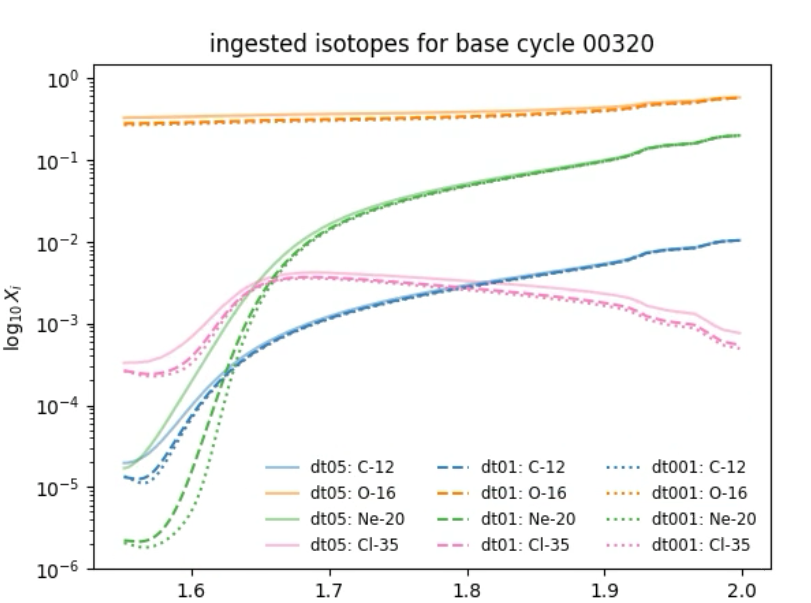
\includegraphics[width=\textwidth]{chapters/1/figures/time_resolution [temp].png}
\caption{TEMP CAPTION
\label{fig:time_resolution}}
\end{figure}

As shown in Figure \ref{fig:time_resolution}, increasing the timestep changes the mass fraction of C-12, O-16, Ne-20, Cl-35.